\section{Results}

\subsection{Single-Turn Results}
% <600-700 words>
\subsubsection{Baseline Single-Turn Performance}
For state representation, the baseline model utilizes:

$$\phi(\mathbf{s}) = \big[\phi_{\mathrm{dice}}^{\mathrm{combined}}(\mathbf{d}), \phi_{\mathrm{cat}}(\mathbf{c}), \phi_{\mathrm{bonus}}(\mathbf{c}), \phi_{\mathrm{rolls}}(r)\big]$$

For outputs, it uses Bernoulli rolling actions and categorical scoring actions.
The single turn model has a short horizon (3 steps); REINFORCE was the natural choice here.
We trained on <X> single-turn episodes, using a batch size of <Y> episodes, for <Z> total gradient updates.

Although it does not nearly reach optimal performance, it performs surprisingly well over the full game; this is likely due to the high correlation between single-turn and full-game optimal actions.
However, we suspected target leakage (selecting parameters and architectures based on full-game performance) could also play a role and analyze the full-game vs. single-turn tradeoff in Section~\ref{sec:tradeoff-curve}.

\begin{figure}[H]
    \centering
    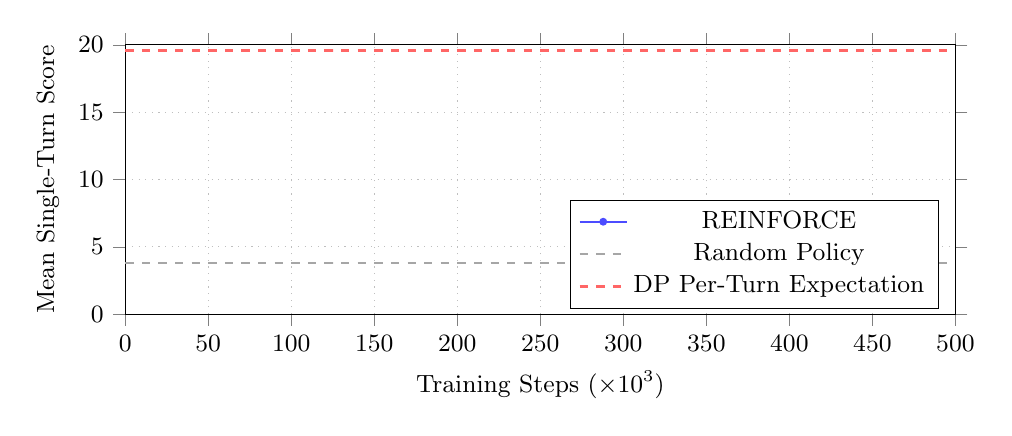
\begin{tikzpicture}
        \begin{axis}[
                width=\columnwidth,
                height=5cm,
                xlabel={Training Steps ($\times 10^3$)},
                ylabel={Mean Single-Turn Score},
                xmin=0, xmax=500,
                ymin=0, ymax=20,
                grid=both,
                grid style={dotted},
                tick align=outside,
                tick label style={font=\small},
                label style={font=\small},
                legend style={at={(0.98,0.02)},anchor=south east,font=\small}
            ]

            % Main REINFORCE learning curve
            \addplot[
                thick,
                blue!70!white,
                mark=*,
                mark size=1pt,
                mark repeat=10
            ] coordinates {
                    (0, 50)
                    (50, 50)
                    (100, 50)
                    (150, 50)
                    (200, 50)
                    (250, 50)
                    (300, 50)
                    (350, 50)
                    (400, 50)
                    (450, 50)
                    (500, 50)
                };
            \addlegendentry{REINFORCE}

            % Random policy baseline
            \addplot[
                dashed,
                gray!70,
                thick,
                domain=0:500
            ] {3.8};
            \addlegendentry{Random Policy}

            % DP per-turn expectation
            \addplot[
                dashed,
                red!60!white,
                thick,
                domain=0:500
            ] {19.59};
            \addlegendentry{DP Per-Turn Expectation}

        \end{axis}
    \end{tikzpicture}
    \caption{Single-turn agent performance during training (placeholder data)}
    \label{fig:single-turn-performance}
\end{figure}

\begin{figure}[H]
    \centering
    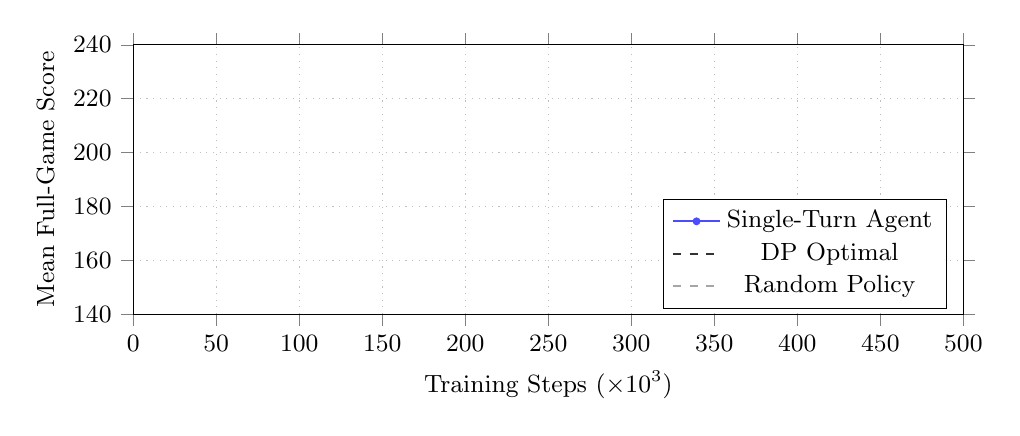
\begin{tikzpicture}
        \begin{axis}[
                width=\columnwidth,
                height=5cm,
                xlabel={Training Steps ($\times 10^3$)},
                ylabel={Mean Full-Game Score},
                xmin=0, xmax=500,
                ymin=140, ymax=240,
                grid=both,
                grid style={dotted},
                tick align=outside,
                tick label style={font=\small},
                label style={font=\small},
                legend style={at={(0.98,0.02)},anchor=south east,font=\small}
            ]

            % Full-game evaluation at checkpoints
            \addplot[
                thick,
                blue!70!white,
                mark=*,
                mark size=1pt,
                mark repeat=10
            ] coordinates {
                    (0, 50)
                    (50, 50)
                    (100, 50)
                    (150, 50)
                    (200, 50)
                    (250, 50)
                    (300, 50)
                    (350, 50)
                    (400, 50)
                    (450, 50)
                    (500, 50)
                };
            \addlegendentry{Single-Turn Agent}

            % DP optimal baseline
            \addplot[
                dashed,
                black!80,
                thick,
                domain=0:500
            ] {254.69};
            \addlegendentry{DP Optimal}

            % Random policy baseline
            \addplot[
                dashed,
                gray!70,
                thick,
                domain=0:500
            ] {49.5};
            \addlegendentry{Random Policy}

        \end{axis}
    \end{tikzpicture}
    \caption{Full-game performance of single-turn agent (placeholder data)}
    \label{fig:single-turn-fullgame}
\end{figure}

\subsubsection{Single vs Full-game Tradeoff Curve}
\label{sec:tradeoff-curve}
To understand the tradeoff between single-turn and full-game performance, we ablated our model using small changes to various hyperparameters and captured
the resulting performance on both the primary single-turn score, as well as the auxiliary full-game score.
We expect that there is a Pareto frontier between these two objectives, and that some hyperparameter choices push performance towards one or the other.

<Pick one:>

<As expected, we can see that full game performance generally increases linearly with single-turn performance.
However, at very high levels of full-game performance, single-turn performance begins to plateau, and even decline slightly.
Since the single-turn model does not have access to the full game context, these are actually imperfectly optimizing their purported objective.
This indicates that selecting hyperparameters for a single-turn model based on full-game performance is indeed a form of target leakage.>

<Contrary to our expectations, we do not see a clear tradeoff between single-turn and full-game performance at high performance levels.
This suggests that single-turn optimization is a good proxy for full-game performance, or that the model is able to reconstruct
sufficient full-game context from the single-turn state representation to make effective long-term decisions.>

\begin{figure}[H]
    \centering
    \begin{tikzpicture}
        \begin{axis}[
            width=\columnwidth,
            xlabel={$\bar{s}_{\text{single-turn}}$},
            ylabel={$\bar{s}_{\text{full-game}}$},
            title={Pareto Frontier of Single-Turn vs. Full-Game Performance},
            grid=both,
            grid style={dotted},
            tick align=outside,
            tick label style={font=\small},
            label style={font=\small},
            title style={font=\small},
            enlargelimits=0.05,
            legend style={at={(0.02,0.98)},anchor=north west,font=\small}
            ]

            % --- Scatter points: replace these with your data ---
            \addplot[
                only marks,
                mark=*,
                blue!70!white,
                mark size=1.5pt
            ] coordinates {
                    (50, 50)
                    (50, 50)
                    (50, 50)
                    (50, 50)
                    (50, 50)
                };
            \addlegendentry{RL configurations}

        \end{axis}
    \end{tikzpicture}
    \caption{Single-turn vs full-game performance (placeholder data)}
    \label{fig:pareto-frontier}
\end{figure}

\subsection{Full-Game Results}
% <600-700 words>
For the full-game model, we added several additional features to the state representation: $\phi_{\mathrm{progress}}(t)$ and $\phi_{\mathrm{potential}}(\mathbf{d}, \mathbf{c})$
while reusing the same underlying neural network architecture as the single-turn model. These additions were necessary to provide the model with sufficient context to make long-term strategic decisions.
While the $\phi_{\mathrm{progress}}(t)$ feature could be inferred from the scorecard, the model struggled to do so reliably.
We intentionally omitted the $\phi_{\mathrm{potential}}(\mathbf{d}, \mathbf{c})$ feature in single turn, as we wanted to ensure the model was capable of learning to reason about category potential on its own,
but found it to be necessary, especially with REINFORCE.

\subsubsection{Algorithm Comparison: REINFORCE, A2C, PPO}

REINFORCE proved challenging to optimize to high performance levels given our fixed training budget of 1 million full-game episodes (39 million steps).
It was highly sensitive to hyperparameters such as the critic coefficient, the entropy bonus, and batch size.
We also found that REINFORCE simply required more training data to converge at a reliable performance level across seeds; our implementation was trained on 1,000,000 games.
However, after optimization we were able to achieve reasonable performance, scoring a mean of <X> points on average over 10,000 full games.

Our most successful algorithm was TD(0)-style Actor-Critic (A2C). We found is easiest to tune and with an immediate performance boost over REINFORCE.
This was the algorithm we use for the ablation studies. With a fixed training budget of 1 million full-games,
A2C was able to approach DP-optimal performance.

We also attempted to use Proximal Policy Optimization (PPO) with TD(0), but found it difficult to tune effectively within our computational budget. Each PPO rollout requires
$k$ epochs of minibatch updates, which significantly increases training time compared to A2C and REINFORCE. Sample efficiency wasn't a huge factor for us, since Yahtzee is so easy to simulate.
For fair comparison to the other algorithms, we had to reduce the total number of games seen during training by a factor of $k$.
However, it is possible PPO could reach or surpass A2C performance with more extensive hyperparameter tuning.

\begin{figure}[H]
    \centering
    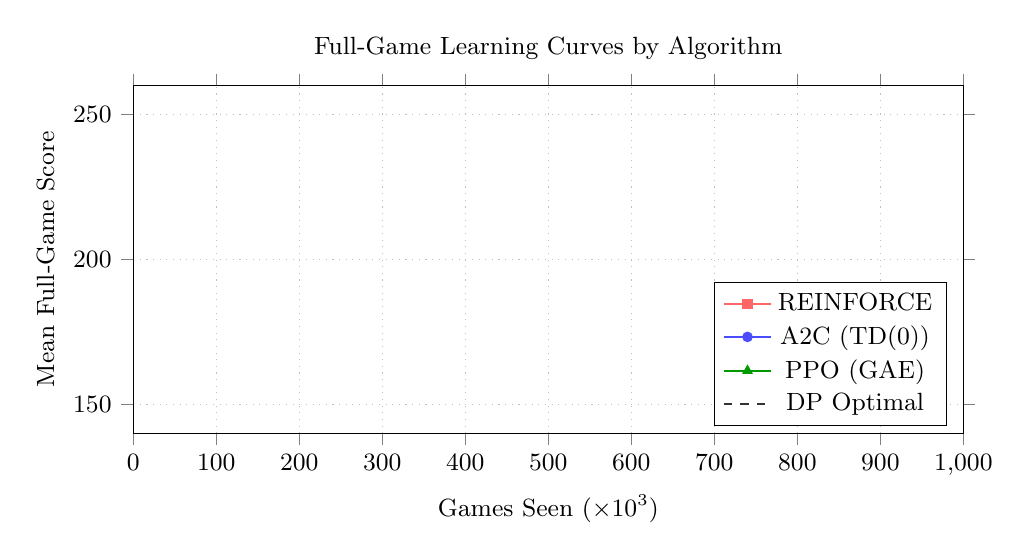
\begin{tikzpicture}
        \begin{axis}[
                width=\columnwidth,
                height=6cm,
                xlabel={Games Seen ($\times 10^3$)},
                ylabel={Mean Full-Game Score},
                title={Full-Game Learning Curves by Algorithm},
                xmin=0, xmax=1000,
                ymin=140, ymax=260,
                grid=both,
                grid style={dotted},
                tick align=outside,
                tick label style={font=\small},
                label style={font=\small},
                title style={font=\small},
                legend style={at={(0.98,0.02)},anchor=south east,font=\small}
            ]

            % REINFORCE learning curve
            \addplot[
                thick,
                red!60!white,
                mark=square*,
                mark size=1.5pt,
                mark repeat=20
            ] coordinates {
                    (0, 50)
                    (100, 50)
                    (200, 50)
                    (300, 50)
                    (400, 50)
                    (500, 50)
                    (600, 50)
                    (700, 50)
                    (800, 50)
                    (900, 50)
                    (1000, 50)
                };
            \addlegendentry{REINFORCE}

            % A2C learning curve
            \addplot[
                thick,
                blue!70!white,
                mark=*,
                mark size=1.5pt,
                mark repeat=20
            ] coordinates {
                    (0, 50)
                    (100, 50)
                    (200, 50)
                    (300, 50)
                    (400, 50)
                    (500, 50)
                    (600, 50)
                    (700, 50)
                    (800, 50)
                    (900, 50)
                    (1000, 50)
                };
            \addlegendentry{A2C (TD(0))}

            % PPO learning curve
            \addplot[
                thick,
                green!60!black,
                mark=triangle*,
                mark size=1.5pt,
                mark repeat=20
            ] coordinates {
                    (0, 50)
                    (100, 50)
                    (200, 50)
                    (300, 50)
                    (400, 50)
                    (500, 50)
                    (600, 50)
                    (700, 50)
                    (800, 50)
                    (900, 50)
                    (1000, 50)
                };
            \addlegendentry{PPO (GAE)}

            % DP optimal baseline
            \addplot[
                dashed,
                black!80,
                thick,
                domain=0:1000
            ] {50};
            \addlegendentry{DP Optimal}

        \end{axis}
    \end{tikzpicture}
    \caption{Algorithm comparison learning curves (placeholder data)}
    \label{fig:full-game-learning-curves}
\end{figure}

\begin{figure}[H]
    \centering
    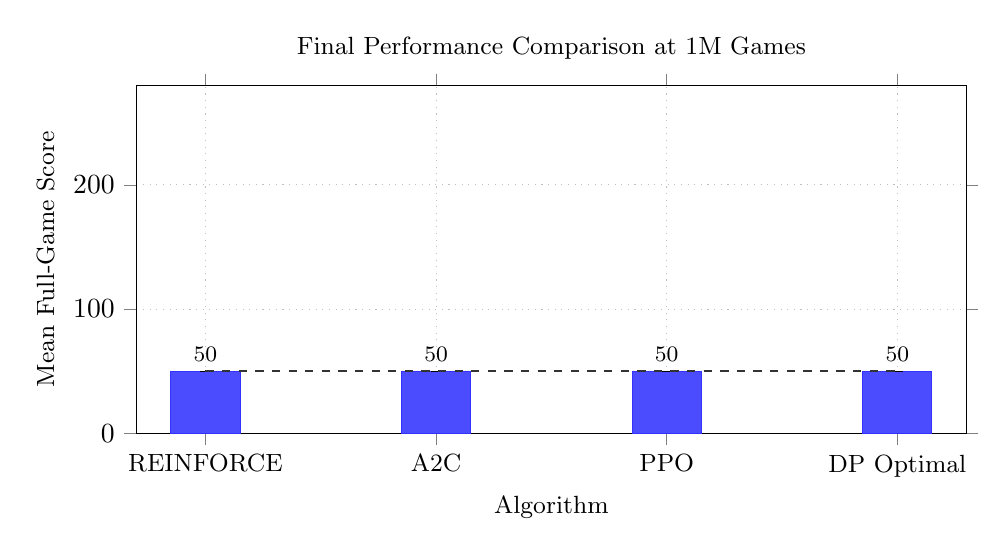
\begin{tikzpicture}
        \begin{axis}[
                ybar,
                width=\columnwidth,
                height=6cm,
                xlabel={Algorithm},
                ylabel={Mean Full-Game Score},
                title={Final Performance Comparison at 1M Games},
                symbolic x coords={REINFORCE, A2C, PPO, DP Optimal},
                xtick=data,
                xticklabel style={font=\small},
                ylabel style={font=\small},
                xlabel style={font=\small},
                title style={font=\small},
                bar width=25pt,
                ymin=0, ymax=280,
                grid=both,
                grid style={dotted},
                tick align=outside,
                nodes near coords,
                nodes near coords style={font=\footnotesize, anchor=south},
            ]

            \addplot[
                fill=blue!70!white,
                draw=blue!80,
                error bars/.cd,
                y dir=both,
                y explicit
            ] coordinates {
                    (REINFORCE, 50) +- (0, 0)
                    (A2C, 50) +- (0, 0)
                    (PPO, 50) +- (0, 0)
                    (DP Optimal, 50) +- (0, 0)
                };

            % Horizontal dashed line at DP optimal
            \draw[dashed, black!80, thick] (axis cs:REINFORCE,50) -- (axis cs:DP Optimal,50);

        \end{axis}
    \end{tikzpicture}
    \caption{Final performance, mean score (placeholder data)}
    \label{fig:final-performance-comparison}
\end{figure}

\begin{figure}[H]
    \centering
    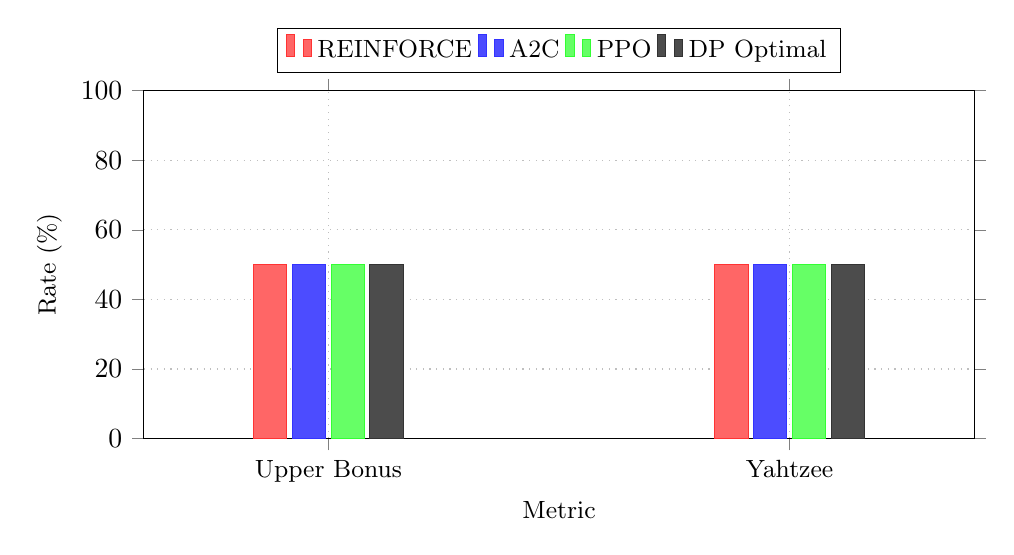
\begin{tikzpicture}
        \begin{axis}[
                ybar,
                width=\columnwidth,
                height=6cm,
                xlabel={Metric},
                ylabel={Rate (\%)},
                title={Bonus and Yahtzee Rates by Algorithm},
                symbolic x coords={Upper Bonus, Yahtzee},
                xtick=data,
                xticklabel style={font=\small},
                ylabel style={font=\small},
                xlabel style={font=\small},
                title style={font=\small},
                ymin=0, ymax=100,
                bar width=12pt,
                grid=both,
                grid style={dotted},
                tick align=outside,
                legend style={at={(0.5,1.05)},anchor=south,legend columns=4,font=\small},
                enlarge x limits=0.4,
            ]

            % REINFORCE
            \addplot[
                fill=red!60!white,
                draw=red!80!white
            ] coordinates {
                    (Upper Bonus, 50)
                    (Yahtzee, 50)
                };
            \addlegendentry{REINFORCE}

            % A2C
            \addplot[
                fill=blue!70!white,
                draw=blue!80!white
            ] coordinates {
                    (Upper Bonus, 50)
                    (Yahtzee, 50)
                };
            \addlegendentry{A2C}

            % PPO
            \addplot[
                fill=green!60!white,
                draw=green!80!white
            ] coordinates {
                    (Upper Bonus, 50)
                    (Yahtzee, 50)
                };
            \addlegendentry{PPO}

            % DP Optimal
            \addplot[
                fill=black!70,
                draw=black!80
            ] coordinates {
                    (Upper Bonus, 50)
                    (Yahtzee, 50)
                };
            \addlegendentry{DP Optimal}

        \end{axis}
    \end{tikzpicture}
    \caption{Bonus and Yahtzee achievement rates (placeholder data)}
    \label{fig:bonus-yahtzee-rates}
\end{figure}

\subsubsection{Representational Ablations}

While a number of additional representational choices were explored, one of the most important is the state representation of the dice.
One important thing to note is that our environment always sorts the dice in ascending order before passing them to the agent.
If this was not done, the network would be forced to waste capacity on understanding permutations of the same dice configuration,
which we found early on was a significant impediment to learning.
<Future work could explore permutation-invariant architectures such as Deep Sets \cite{zaheer-2017-deep-sets} or embeddings with self-attention to handle unsorted dice.>

We wanted to highlight the importance of using a combined representation of both one-hot encodings and counts-based encodings of the dice.
While the network could theoretically learn to reconstruct either representation from the other, in practice we found that using both improved performance.

\begin{figure}[H]
    \centering
    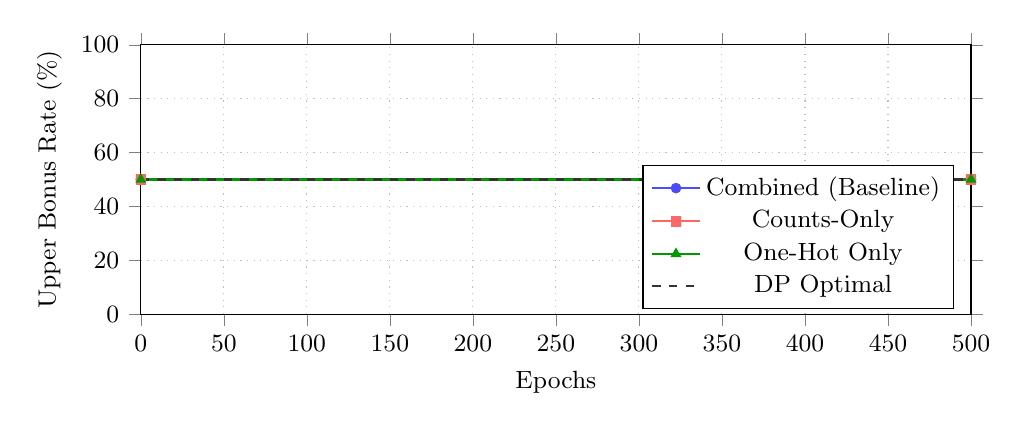
\begin{tikzpicture}
        \begin{axis}[
                width=\columnwidth,
                height=5cm,
                xlabel={Epochs},
                ylabel={Upper Bonus Rate (\%)},
                xmin=0, xmax=500,
                ymin=0, ymax=100,
                grid=both,
                grid style={dotted},
                tick align=outside,
                tick label style={font=\small},
                label style={font=\small},
                legend style={at={(0.98,0.02)},anchor=south east,font=\small}
            ]

            % Combined (baseline)
            \addplot[
                thick,
                blue!70!white,
                mark=*,
                mark size=1.5pt,
                mark repeat=10
            ] coordinates {
                    (0, 50)
                    (50, 50)
                    (100, 50)
                    (150, 50)
                    (200, 50)
                    (250, 50)
                    (300, 50)
                    (350, 50)
                    (400, 50)
                    (450, 50)
                    (500, 50)
                };
            \addlegendentry{Combined (Baseline)}

            % Counts-only
            \addplot[
                thick,
                red!60!white,
                mark=square*,
                mark size=1.5pt,
                mark repeat=10
            ] coordinates {
                    (0, 50)
                    (50, 50)
                    (100, 50)
                    (150, 50)
                    (200, 50)
                    (250, 50)
                    (300, 50)
                    (350, 50)
                    (400, 50)
                    (450, 50)
                    (500, 50)
                };
            \addlegendentry{Counts-Only}

            % One-hot only
            \addplot[
                thick,
                green!60!black,
                mark=triangle*,
                mark size=1.5pt,
                mark repeat=10
            ] coordinates {
                    (0, 50)
                    (50, 50)
                    (100, 50)
                    (150, 50)
                    (200, 50)
                    (250, 50)
                    (300, 50)
                    (350, 50)
                    (400, 50)
                    (450, 50)
                    (500, 50)
                };
            \addlegendentry{One-Hot Only}

            % DP optimal baseline
            \addplot[
                dashed,
                black!80,
                thick,
                domain=0:500
            ] {50};
            \addlegendentry{DP Optimal}

        \end{axis}
    \end{tikzpicture}
    \caption{Upper bonus achievement by dice representation (placeholder data)}
    \label{fig:dice-representation-bonus}
\end{figure}

For the full-game model, we added several additional features beyond the single-turn representation.
To understand the importance of each, they were ablated individually.

\begin{figure}[H]
    \centering
    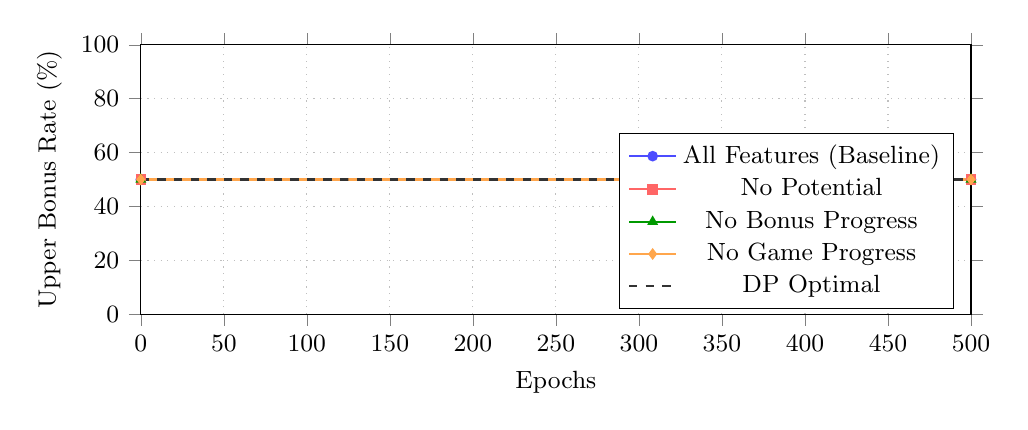
\begin{tikzpicture}
        \begin{axis}[
                width=\columnwidth,
                height=5cm,
                xlabel={Epochs},
                ylabel={Upper Bonus Rate (\%)},
                xmin=0, xmax=500,
                ymin=0, ymax=100,
                grid=both,
                grid style={dotted},
                tick align=outside,
                tick label style={font=\small},
                label style={font=\small},
                legend style={at={(0.98,0.02)},anchor=south east,font=\small}
            ]

            % All features (baseline)
            \addplot[
                thick,
                blue!70!white,
                mark=*,
                mark size=1.5pt,
                mark repeat=10
            ] coordinates {
                    (0, 50)
                    (50, 50)
                    (100, 50)
                    (150, 50)
                    (200, 50)
                    (250, 50)
                    (300, 50)
                    (350, 50)
                    (400, 50)
                    (450, 50)
                    (500, 50)
                };
            \addlegendentry{All Features (Baseline)}

            % No potential
            \addplot[
                thick,
                red!60!white,
                mark=square*,
                mark size=1.5pt,
                mark repeat=10
            ] coordinates {
                    (0, 50)
                    (50, 50)
                    (100, 50)
                    (150, 50)
                    (200, 50)
                    (250, 50)
                    (300, 50)
                    (350, 50)
                    (400, 50)
                    (450, 50)
                    (500, 50)
                };
            \addlegendentry{No Potential}

            % No bonus progress
            \addplot[
                thick,
                green!60!black,
                mark=triangle*,
                mark size=1.5pt,
                mark repeat=10
            ] coordinates {
                    (0, 50)
                    (50, 50)
                    (100, 50)
                    (150, 50)
                    (200, 50)
                    (250, 50)
                    (300, 50)
                    (350, 50)
                    (400, 50)
                    (450, 50)
                    (500, 50)
                };
            \addlegendentry{No Bonus Progress}

            % No game progress
            \addplot[
                thick,
                orange!70!white,
                mark=diamond*,
                mark size=1.5pt,
                mark repeat=10
            ] coordinates {
                    (0, 50)
                    (50, 50)
                    (100, 50)
                    (150, 50)
                    (200, 50)
                    (250, 50)
                    (300, 50)
                    (350, 50)
                    (400, 50)
                    (450, 50)
                    (500, 50)
                };
            \addlegendentry{No Game Progress}

            % DP optimal baseline
            \addplot[
                dashed,
                black!80,
                thick,
                domain=0:500
            ] {50};
            \addlegendentry{DP Optimal}

        \end{axis}
    \end{tikzpicture}
    \caption{Upper bonus achievement by feature ablation (placeholder data)}
    \label{fig:feature-ablation-bonus}
\end{figure}

\subsubsection{Architectural Ablations}

We performed a simple grid search ablation to understand if our chosen architecture of 3 hidden layers of 600 units each was optimal.
Yahtzee is a fairly complex game, so we expected shorter, but wider networks to perform best. Note that each of these has a different number of total parameters,
so this is not a pure ablation of depth vs. width.

\begin{figure}[H]
    \centering
    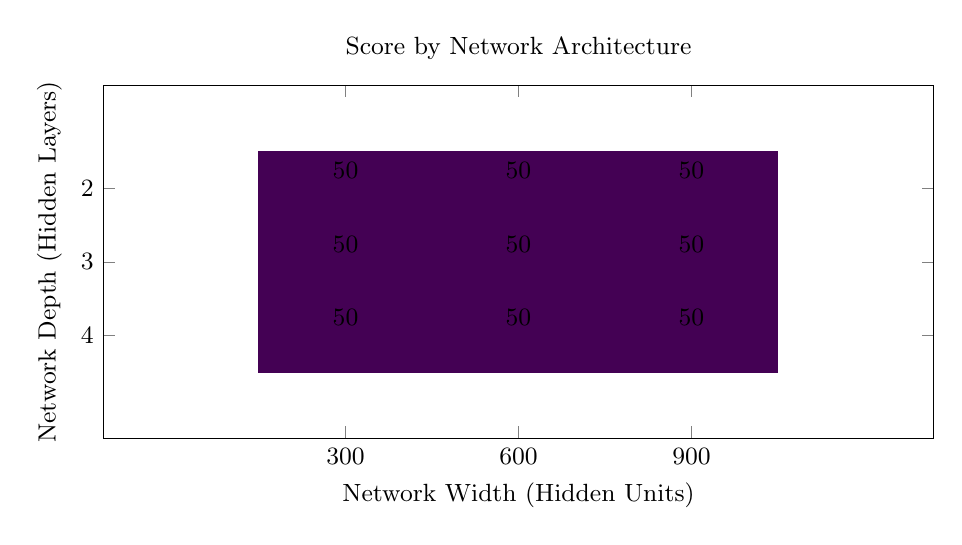
\begin{tikzpicture}
        \begin{axis}[
                width=\columnwidth,
                height=0.5\textwidth,
                xlabel={Network Width (Hidden Units)},
                ylabel={Network Depth (Hidden Layers)},
                title={Score by Network Architecture},
                colormap/viridis,
                xlabel style={font=\small},
                ylabel style={font=\small},
                title style={font=\small},
                xtick={1,2,3},
                xticklabels={300, 600, 900},
                ytick={1,2,3},
                yticklabels={2, 3, 4},
                xticklabel style={font=\small},
                yticklabel style={font=\small},
                enlargelimits=0.3,
                point meta min=230,
                point meta max=245,
                nodes near coords,
                nodes near coords style={font=\small, color=black},
                every node near coord/.append style={xshift=0pt, yshift=0pt},
            ]

            \addplot[
                matrix plot,
                mesh/cols=3,
                point meta=explicit
            ] table[meta=score] {
                    x y score
                    1 1 50
                    2 1 50
                    3 1 50
                    1 2 50
                    2 2 50
                    3 2 50
                    1 3 50
                    2 3 50
                    3 3 50
                };

        \end{axis}
    \end{tikzpicture}
    \caption{Network architecture ablation (placeholder data)}
    \label{fig:architecture-heatmap}
\end{figure}

Based on \cite{bjorck-2022-high-variance}, we hypothesized that Layer Normalization \cite{ba-2016-layer-norm} would improve training stability and performance
and used it in all of our main experiments. This was ablated to understand its true impact.

\begin{figure}[H]
    \centering
    % Panel (a): Learning curves
    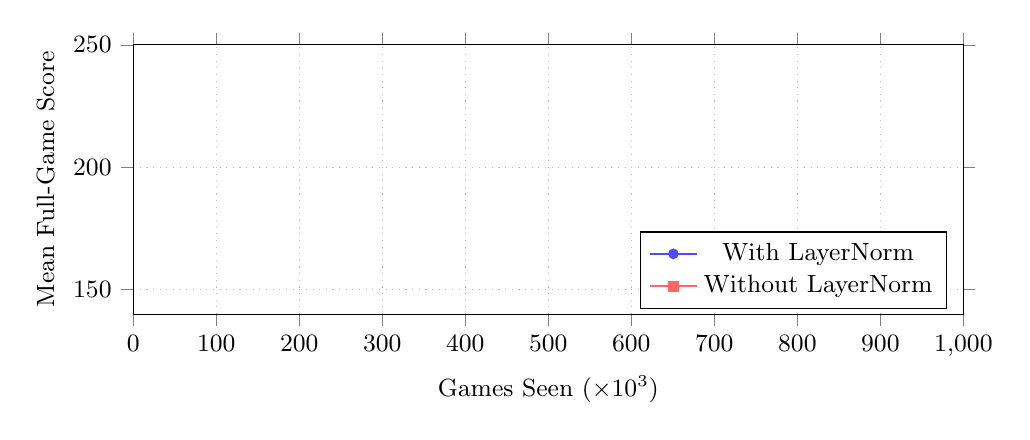
\begin{tikzpicture}
        \begin{axis}[
                width=\columnwidth,
                height=5cm,
                xlabel={Games Seen ($\times 10^3$)},
                ylabel={Mean Full-Game Score},
                xmin=0, xmax=1000,
                ymin=140, ymax=250,
                grid=both,
                grid style={dotted},
                tick align=outside,
                tick label style={font=\small},
                label style={font=\small},
                legend style={at={(0.98,0.02)},anchor=south east,font=\small}
            ]

            % With LayerNorm
            \addplot[
                thick,
                blue!70!white,
                mark=*,
                mark size=1.5pt,
                mark repeat=20
            ] coordinates {
                    (0, 50)
                    (100, 50)
                    (200, 50)
                    (300, 50)
                    (400, 50)
                    (500, 50)
                    (600, 50)
                    (700, 50)
                    (800, 50)
                    (900, 50)
                    (1000, 50)
                };
            \addlegendentry{With LayerNorm}

            % Without LayerNorm
            \addplot[
                thick,
                red!60!white,
                mark=square*,
                mark size=1.5pt,
                mark repeat=20
            ] coordinates {
                    (0, 50)
                    (100, 50)
                    (200, 50)
                    (300, 50)
                    (400, 50)
                    (500, 50)
                    (600, 50)
                    (700, 50)
                    (800, 50)
                    (900, 50)
                    (1000, 50)
                };
            \addlegendentry{Without LayerNorm}

        \end{axis}
    \end{tikzpicture}
    \caption{Learning curves with and without LayerNorm (placeholder data)}
    \label{fig:layernorm-learning}
\end{figure}

\begin{figure}[H]
    \centering
    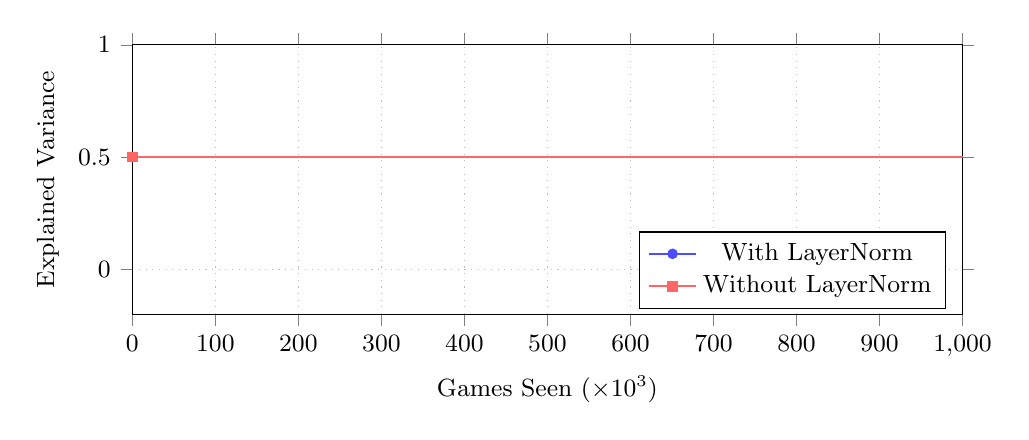
\begin{tikzpicture}
        \begin{axis}[
                width=\columnwidth,
                height=5cm,
                xlabel={Games Seen ($\times 10^3$)},
                ylabel={Explained Variance},
                xmin=0, xmax=1000,
                ymin=-0.2, ymax=1.0,
                grid=both,
                grid style={dotted},
                tick align=outside,
                tick label style={font=\small},
                label style={font=\small},
                legend style={at={(0.98,0.02)},anchor=south east,font=\small}
            ]

            % With LayerNorm
            \addplot[
                thick,
                blue!70!white,
                mark=*,
                mark size=1.5pt,
                mark repeat=20
            ] coordinates {
                    (0, 0.5)
                    (100, 0.5)
                    (200, 0.5)
                    (300, 0.5)
                    (400, 0.5)
                    (500, 0.5)
                    (600, 0.5)
                    (700, 0.5)
                    (800, 0.5)
                    (900, 0.5)
                    (1000, 0.5)
                };
            \addlegendentry{With LayerNorm}

            % Without LayerNorm
            \addplot[
                thick,
                red!60!white,
                mark=square*,
                mark size=1.5pt,
                mark repeat=20
            ] coordinates {
                    (0, 0.5)
                    (100, 0.5)
                    (200, 0.5)
                    (300, 0.5)
                    (400, 0.5)
                    (500, 0.5)
                    (600, 0.5)
                    (700, 0.5)
                    (800, 0.5)
                    (900, 0.5)
                    (1000, 0.5)
                };
            \addlegendentry{Without LayerNorm}

        \end{axis}
    \end{tikzpicture}
    \caption{Value function quality with and without LayerNorm (placeholder data)}
    \label{fig:layernorm-value}
\end{figure}

Lastly, we used SILU activation functions in our network for all of our main experiments, as it had been reported to work well in RL settings \cite{henderson-2021-silu-rl}.
We ablated this to ReLU to understand its true impact.

\begin{figure}[H]
    \centering
    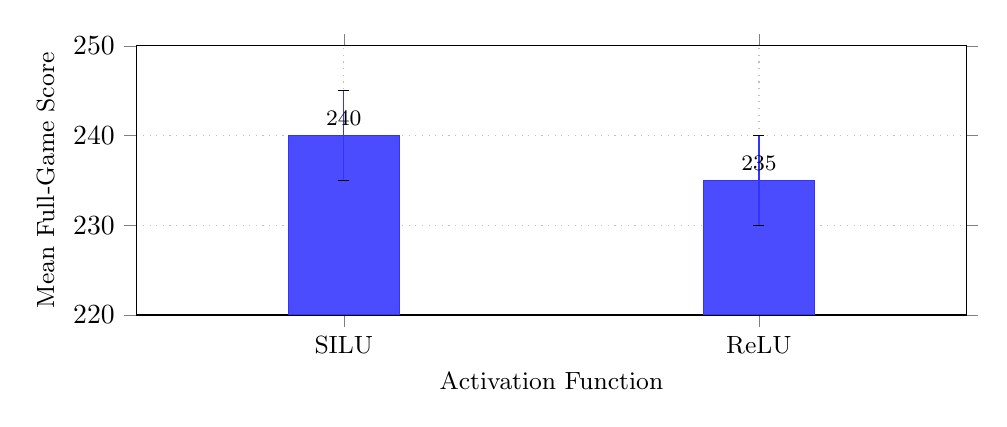
\begin{tikzpicture}
        \begin{axis}[
                ybar,
                width=\columnwidth,
                height=5cm,
                xlabel={Activation Function},
                ylabel={Mean Full-Game Score},
                symbolic x coords={SILU, ReLU},
                xtick=data,
                xticklabel style={font=\small},
                ylabel style={font=\small},
                xlabel style={font=\small},
                bar width=40pt,
                ymin=220, ymax=250,
                grid=both,
                grid style={dotted},
                tick align=outside,
                nodes near coords,
                nodes near coords style={font=\footnotesize, anchor=south},
                enlarge x limits=0.5,
            ]

            \addplot[
                fill=blue!70!white,
                draw=blue!80,
                error bars/.cd,
                y dir=both,
                y explicit
            ] coordinates {
                    (SILU, 240) +- (0, 5)
                    (ReLU, 235) +- (0, 5)
                };

        \end{axis}
    \end{tikzpicture}
    \caption{Performance comparison: SILU vs ReLU activation (placeholder data)}
    \label{fig:silu-vs-relu}
\end{figure}

\subsubsection{Credit Assignment: TD(0) vs GAE}

Later in this research, we noticed the main issue with our network was that it was struggling to earn the bonus, learning it very slowly.
We first hypothesized that this was due to high variance in REINFORCE, so we switched to A2C with TD(0) targets. However, the issue
persisted. We then hypothesized that the TD(0) targets were not providing sufficient credit assignment for the long-term bonus reward,
so we switched to GAE with various $\lambda$ values to understand if this would help.

Unfortunately, we found that GAE did not improve performance over TD(0), and values that were too high ($\lambda \geq 0.8$)
significantly degraded performance.

\begin{figure}[H]
    \centering
    % Panel (a): Mean score vs lambda
    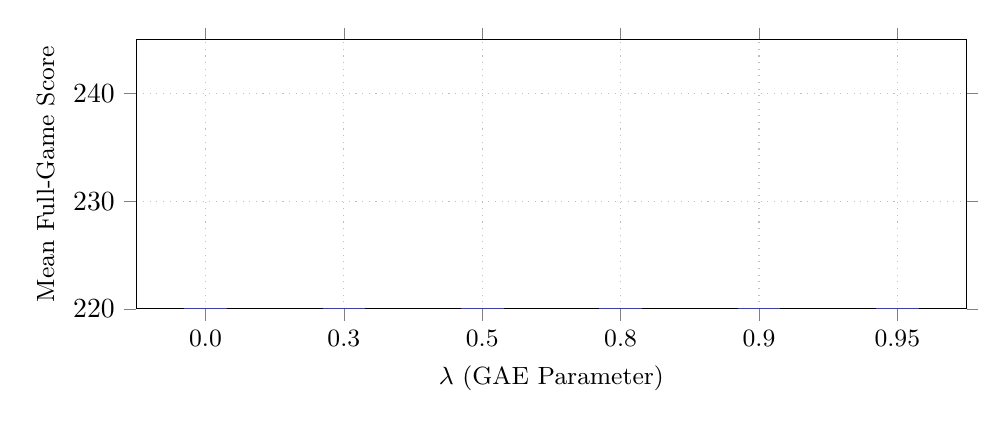
\begin{tikzpicture}
        \begin{axis}[
                ybar,
                width=\columnwidth,
                height=5cm,
                xlabel={$\lambda$ (GAE Parameter)},
                ylabel={Mean Full-Game Score},
                symbolic x coords={0.0, 0.3, 0.5, 0.8, 0.9, 0.95},
                xtick=data,
                xticklabel style={font=\small},
                ylabel style={font=\small},
                xlabel style={font=\small},
                bar width=15pt,
                ymin=220, ymax=245,
                grid=both,
                grid style={dotted},
                tick align=outside,
                nodes near coords,
                nodes near coords style={font=\footnotesize, anchor=south},
            ]

            \addplot[
                fill=blue!70!white,
                draw=blue!80!white,
                error bars/.cd,
                y dir=both,
                y explicit
            ] coordinates {
                    (0.0, 50) +- (0, 0)
                    (0.3, 50) +- (0, 0)
                    (0.5, 50) +- (0, 0)
                    (0.8, 50) +- (0, 0)
                    (0.9, 50) +- (0, 0)
                    (0.95, 50) +- (0, 0)
                };

        \end{axis}
    \end{tikzpicture}
    \caption{Final performance by GAE lambda (placeholder data)}
    \label{fig:gae-lambda-performance}
\end{figure}

\begin{figure}[H]
    \centering
    \begin{tikzpicture}
        \begin{axis}[
                ybar,
                width=\columnwidth,
                height=5cm,
                xlabel={$\lambda$ (GAE Parameter)},
                ylabel={Upper Bonus Rate (\%)},
                symbolic x coords={0.0, 0.3, 0.5, 0.8, 0.9, 0.95},
                xtick=data,
                xticklabel style={font=\small},
                ylabel style={font=\small},
                xlabel style={font=\small},
                bar width=15pt,
                ymin=60, ymax=85,
                grid=both,
                grid style={dotted},
                tick align=outside,
                nodes near coords,
                nodes near coords style={font=\footnotesize, anchor=south},
            ]

            \addplot[
                fill=green!60!white,
                draw=green!80!white,
                error bars/.cd,
                y dir=both,
                y explicit
            ] coordinates {
                    (0.0, 50) +- (0, 0)
                    (0.3, 50) +- (0, 0)
                    (0.5, 50) +- (0, 0)
                    (0.8, 50) +- (0, 0)
                    (0.9, 50) +- (0, 0)
                    (0.95, 50) +- (0, 0)
                };

        \end{axis}
    \end{tikzpicture}
    \caption{Upper bonus achievement by GAE lambda (placeholder data)}
    \label{fig:gae-lambda-bonus}
\end{figure}

\subsubsection{Entropy Sensitivity}
During experimentation, we noticed that the entropy regularization coefficients had a significant impact on training stability and final performance.
With no regularization, the policy quickly converges to a deterministic policy that fails to explore sufficiently.
With too much regularization, the policy would not perform well enough to quickly learn strategies for earning Yahtzee's and the bonus.
To better understand this sensitivity, we trained models under three different entropy regimes: Low Entropy, Baseline, and High Entropy.

\begin{table}[H]
    \centering
    \small
    \caption{Entropy regime definitions}
    \label{tab:entropy-regime-definitions}
    \begin{tabular}{lcc}
        \hline
        \textbf{Regime} & $\beta_{\mathrm{roll}}$   & $\beta_{\mathrm{score}}$ \\
        \hline
        Low Entropy     & 0.005 $\rightarrow$ 0.001 & 0.01 $\rightarrow$ 0.002 \\
        Baseline        & 0.01 $\rightarrow$ 0.002  & 0.02 $\rightarrow$ 0.005 \\
        High Entropy    & 0.02 $\rightarrow$ 0.005  & 0.04 $\rightarrow$ 0.01  \\
        \hline
    \end{tabular}
\end{table}

\begin{figure}[H]
    \centering
    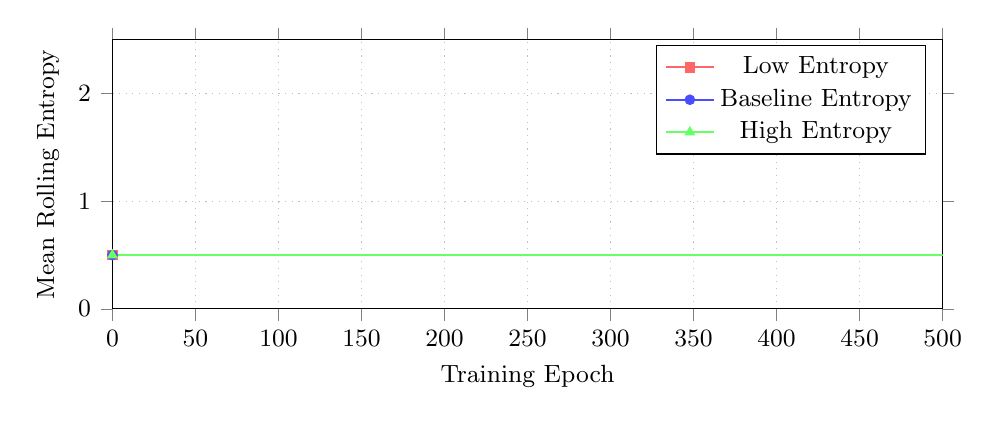
\begin{tikzpicture}
        \begin{axis}[
                width=\columnwidth,
                height=5cm,
                xlabel={Training Epoch},
                ylabel={Mean Rolling Entropy},
                xmin=0, xmax=500,
                ymin=0, ymax=2.5,
                grid=both,
                grid style={dotted},
                tick align=outside,
                tick label style={font=\small},
                label style={font=\small},
                legend style={at={(0.98,0.98)},anchor=north east,font=\small}
            ]

            % Low entropy
            \addplot[
                thick,
                red!60!white,
                mark=square*,
                mark size=1.5pt,
                mark repeat=20
            ] coordinates {
                    (0, 0.5)
                    (50, 0.5)
                    (100, 0.5)
                    (150, 0.5)
                    (200, 0.5)
                    (250, 0.5)
                    (300, 0.5)
                    (350, 0.5)
                    (400, 0.5)
                    (450, 0.5)
                    (500, 0.5)
                };
            \addlegendentry{Low Entropy}

            % Baseline entropy
            \addplot[
                thick,
                blue!70!white,
                mark=*,
                mark size=1.5pt,
                mark repeat=20
            ] coordinates {
                    (0, 0.5)
                    (50, 0.5)
                    (100, 0.5)
                    (150, 0.5)
                    (200, 0.5)
                    (250, 0.5)
                    (300, 0.5)
                    (350, 0.5)
                    (400, 0.5)
                    (450, 0.5)
                    (500, 0.5)
                };
            \addlegendentry{Baseline Entropy}

            % High entropy
            \addplot[
                thick,
                green!60!white,
                mark=triangle*,
                mark size=1.5pt,
                mark repeat=20
            ] coordinates {
                    (0, 0.5)
                    (50, 0.5)
                    (100, 0.5)
                    (150, 0.5)
                    (200, 0.5)
                    (250, 0.5)
                    (300, 0.5)
                    (350, 0.5)
                    (400, 0.5)
                    (450, 0.5)
                    (500, 0.5)
                };
            \addlegendentry{High Entropy}

        \end{axis}
    \end{tikzpicture}
    \caption{Rolling-head entropy over training (placeholder data)}
    \label{fig:entropy-rolling}
\end{figure}

\begin{figure}[H]
    \centering
    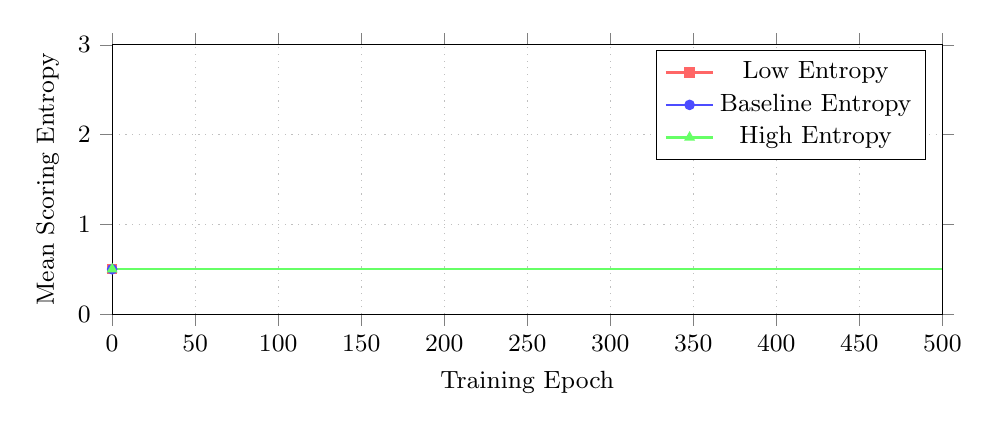
\begin{tikzpicture}
        \begin{axis}[
                width=\columnwidth,
                height=5cm,
                xlabel={Training Epoch},
                ylabel={Mean Scoring Entropy},
                xmin=0, xmax=500,
                ymin=0, ymax=3.0,
                grid=both,
                grid style={dotted},
                tick align=outside,
                tick label style={font=\small},
                label style={font=\small},
                legend style={at={(0.98,0.98)},anchor=north east,font=\small}
            ]

            % Low entropy
            \addplot[
                thick,
                red!60!white,
                mark=square*,
                mark size=1.5pt,
                mark repeat=20
            ] coordinates {
                    (0, 0.5)
                    (50, 0.5)
                    (100, 0.5)
                    (150, 0.5)
                    (200, 0.5)
                    (250, 0.5)
                    (300, 0.5)
                    (350, 0.5)
                    (400, 0.5)
                    (450, 0.5)
                    (500, 0.5)
                };
            \addlegendentry{Low Entropy}

            % Baseline entropy
            \addplot[
                thick,
                blue!70!white,
                mark=*,
                mark size=1.5pt,
                mark repeat=20
            ] coordinates {
                    (0, 0.5)
                    (50, 0.5)
                    (100, 0.5)
                    (150, 0.5)
                    (200, 0.5)
                    (250, 0.5)
                    (300, 0.5)
                    (350, 0.5)
                    (400, 0.5)
                    (450, 0.5)
                    (500, 0.5)
                };
            \addlegendentry{Baseline Entropy}

            % High entropy
            \addplot[
                thick,
                green!60!white,
                mark=triangle*,
                mark size=1.5pt,
                mark repeat=20
            ] coordinates {
                    (0, 0.5)
                    (50, 0.5)
                    (100, 0.5)
                    (150, 0.5)
                    (200, 0.5)
                    (250, 0.5)
                    (300, 0.5)
                    (350, 0.5)
                    (400, 0.5)
                    (450, 0.5)
                    (500, 0.5)
                };
            \addlegendentry{High Entropy}

        \end{axis}
    \end{tikzpicture}
    \caption{Scoring-head entropy over training (placeholder data)}
    \label{fig:entropy-scoring}
\end{figure}

\begin{table}[H]
    \centering
    \small
    \caption{Entropy regime performance (placeholder data)}
    \label{tab:entropy-regimes}
    \begin{tabular}{lccc}
        \hline
        \textbf{Regime} & \textbf{Mean Score} & \textbf{Bonus \%} & \textbf{Yahtzee \%} \\
        \hline
        Low Entropy     & $<X> \pm <Y>$       & <X>               & <Y>                 \\
        Baseline        & $<X> \pm <Y>$       & <X>               & <Y>                 \\
        High Entropy    & $<X> \pm <Y>$       & <X>               & <Y>                 \\
        \hline
    \end{tabular}
\end{table}

\subsubsection{Summary}
In summary, we found that A2C with TD(0) targets, a combined dice representation, Layer Normalization, SILU activations,
and carefully tuned entropy regularization produced the best results.

\begin{table*}[t]
    \centering
    \small
    \caption{Full-game performance summary (placeholder data)}
    \label{tab:full-game-summary}
    \begin{tabular}{lcccccc}
        \hline
        \textbf{Algorithm}         & \textbf{Training Budget} & \textbf{Mean Score} & \textbf{Std Dev} & \textbf{Bonus Rate (\%)} & \textbf{Yahtzee Rate (\%)} & \textbf{$\geq$250 (\%)} \\
        \hline
        DP Optimal                 & --                       & $<X>$               & --               & $<X>$                    & $<Y>$                      & $<Z>$                   \\
        A2C                        & 250K games               & $<X>$               & $<Y>$            & $<X>$                    & $<Y>$                      & $<Z>$                   \\
        A2C                        & 1M games                 & $<X>$               & $<Y>$            & $<X>$                    & $<Y>$                      & $<Z>$                   \\
        A2C (lower entropy floor)  & 5M games                 & $<X>$               & $<Y>$            & $<X>$                    & $<Y>$                      & $<Z>$                   \\
        PPO ($\lambda=0.3$, $k=3$) & 250K games               & $<X>$               & $<Y>$            & $<X>$                    & $<Y>$                      & $<Z>$                   \\
        REINFORCE (full-game)      & 250K games               & $<X>$               & $<Y>$            & $<X>$                    & $<Y>$                      & $<Z>$                   \\
        REINFORCE (full-game)      & 1M games                 & $<X>$               & $<Y>$            & $<X>$                    & $<Y>$                      & $<Z>$                   \\
        REINFORCE (single-turn)    & 500K games               & $<X>$               & $<Y>$            & $<X>$                    & $<Y>$                      & $<Z>$                   \\
        \hline
    \end{tabular}
\end{table*}

For our best configuration, A2C trained over 5,000,000 games, the final score distribution is compared to DP-optimal in Table \ref{tab:dp-score-distribution}.
\begin{table}[H]
    \centering
    \small
    \caption{Score distribution (placeholder data)}
    \label{tab:dp-score-distribution}
    \begin{tabular}{cc}
        \hline
        \textbf{$n$} & \textbf{$P(\text{score} \geq n)$} \\
        \hline
        50           & $<X>$                             \\
        100          & $<X>$                             \\
        150          & $<X>$                             \\
        200          & $<X>$                             \\
        250          & $<X>$                             \\
        300          & $<X>$                             \\
        400          & $<X>$                             \\
        500          & $<X>$                             \\
        750          & $<X>$                             \\
        1000         & $<X>$                             \\
        1250         & $<X>$                             \\
        1500         & $<X>$                             \\
        \hline
    \end{tabular}
\end{table}

\subsection{Policy Analysis}
% <300-500 words>
\subsubsection{Category Usage}
To understand the overall performance of the agents, we compare their average scores in each category as a percentage of the DP-optimal score for that category
in figures \ref{fig:category-upper} and \ref{fig:category-lower}.

The primary differentiators between our RL agents and the DP optimal solution are in the upper section (and bonus), four-of-a-kind and Yahtzee.
Performance in the upper section is critical to achieving a high overall score, as it enables the bonus however it appears to be traded off against
the four-of-a-kind; it seems the agents prefer to take the immediate points from the 5th die rather than place themselves in a safer position to earn the bonus later.

Yahtzee's high performance was interesting; it requires agents to be performing at a competent level across a single turn in order to earn. We contrast the learning
curve of the Yahtzee category with that of the upper bonus in Figure <INSERT A FIGURE FOR THIS>. The interesting takeaway here is that agents appear to
exhibit a "mode shift" in their strategy once they figure out Yahtzee, whereas the bonus is learned more gradually over time.

\begin{figure}[H]
    \centering
    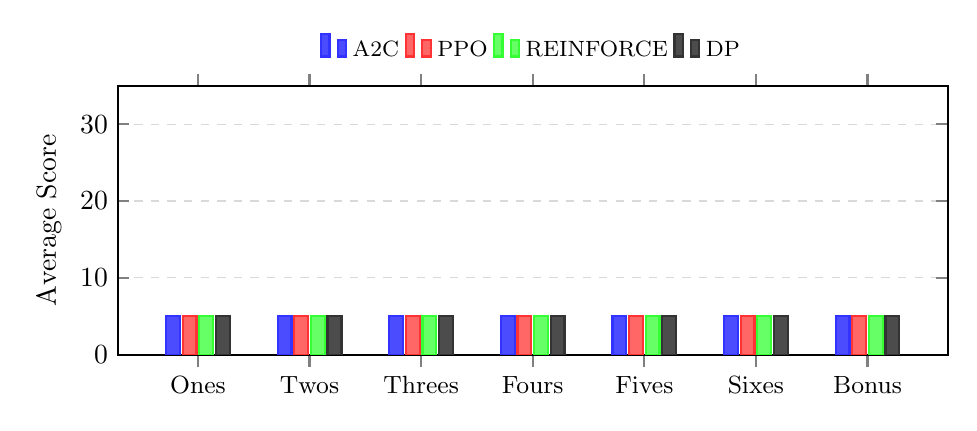
\begin{tikzpicture}
        \begin{axis}[
                ybar=1pt,
                width=\columnwidth,
                height=5cm,
                bar width=5pt,
                symbolic x coords={Ones,Twos,Threes,Fours,Fives,Sixes,Bonus},
                xtick=data,
                xticklabel style={font=\small},
                ylabel={Average Score},
                ymin=0,
                ymax=35,
                ymajorgrids=true,
                grid style={dashed,gray!30},
                legend style={
                        at={(0.5,1.05)},
                        anchor=south,
                        legend columns=4,
                        font=\footnotesize,
                        draw=none,
                        fill=none
                    },
                enlarge x limits=0.12,
                axis line style={thick},
                tick style={thick},
            ]

            % A2C
            \addplot[fill=blue!70!white, draw=blue!80!white, thick] coordinates {
                    (Ones,   5) (Twos,   5) (Threes, 5) (Fours,  5)
                    (Fives,  5) (Sixes,  5) (Bonus,  5)
                };

            % PPO
            \addplot[fill=red!60!white, draw=red!80!white, thick] coordinates {
                    (Ones,   5) (Twos,   5) (Threes, 5) (Fours,  5)
                    (Fives,  5) (Sixes,  5) (Bonus,  5)
                };

            % REINFORCE
            \addplot[fill=green!60!white, draw=green!80!white, thick] coordinates {
                    (Ones,   5) (Twos,   5) (Threes, 5) (Fours,  5)
                    (Fives,  5) (Sixes,  5) (Bonus,  5)
                };

            % DP
            \addplot[fill=black!70, draw=black!80, thick] coordinates {
                    (Ones,   5) (Twos,   5) (Threes, 5) (Fours,  5)
                    (Fives,  5) (Sixes,  5) (Bonus,  5)
                };

            \legend{A2C,PPO,REINFORCE,DP}

        \end{axis}
    \end{tikzpicture}
    \caption{Upper section and bonus scores (placeholder data)}
    \label{fig:category-upper}
\end{figure}

\begin{figure}[H]
    \centering
    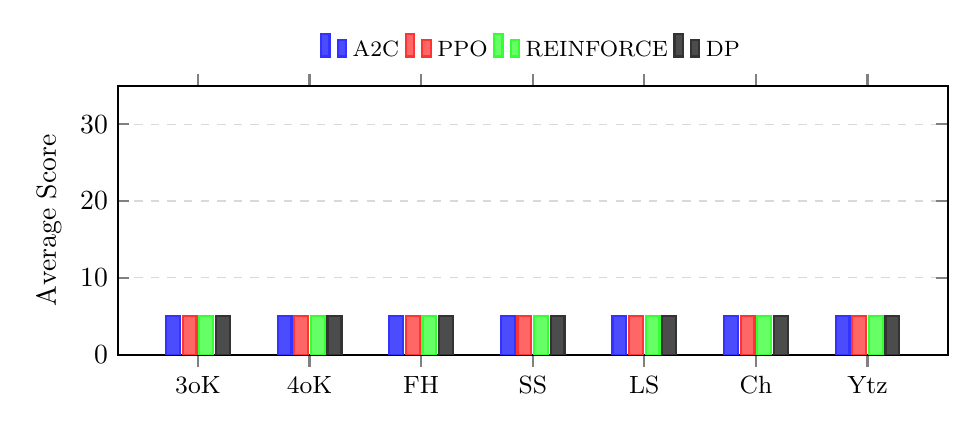
\begin{tikzpicture}
        \begin{axis}[
                ybar=1pt,
                width=\columnwidth,
                height=5cm,
                bar width=5pt,
                symbolic x coords={3oK,4oK,FH,SS,LS,Ch,Ytz},
                xtick=data,
                xticklabel style={font=\small},
                ylabel={Average Score},
                ymin=0,
                ymax=35,
                ymajorgrids=true,
                grid style={dashed,gray!30},
                legend style={
                        at={(0.5,1.05)},
                        anchor=south,
                        legend columns=4,
                        font=\footnotesize,
                        draw=none,
                        fill=none
                    },
                enlarge x limits=0.12,
                axis line style={thick},
                tick style={thick},
            ]

            % A2C
            \addplot[fill=blue!70!white, draw=blue!80!white, thick] coordinates {
                    (3oK,  5) (4oK,  5) (FH,   5) (SS,   5)
                    (LS,   5) (Ch,   5) (Ytz,  5)
                };

            % PPO
            \addplot[fill=red!60!white, draw=red!80!white, thick] coordinates {
                    (3oK,  5) (4oK,  5) (FH,   5) (SS,   5)
                    (LS,   5) (Ch,   5) (Ytz,  5)
                };

            % REINFORCE
            \addplot[fill=green!60!white, draw=green!80!white, thick] coordinates {
                    (3oK,  5) (4oK,  5) (FH,   5) (SS,   5)
                    (LS,   5) (Ch,   5) (Ytz,  5)
                };

            % DP
            \addplot[fill=black!70, draw=black!80, thick] coordinates {
                    (3oK,  5) (4oK,  5) (FH,   5) (SS,   5)
                    (LS,   5) (Ch,   5) (Ytz,  5)
                };

            \legend{A2C,PPO,REINFORCE,DP}

        \end{axis}
    \end{tikzpicture}
    \caption{Lower section scores (placeholder data)}
    \label{fig:category-lower}
\end{figure}

\subsubsection{Strategy Comparison Across Agents}
We also compared some high-level strategy metrics across our different agents to understand how their learned policies differed.
First, we analyzed the distribution of the first category choice made by each agent in Figure \ref{fig:strategy-first-category}.
Next, we analyzed each category to understand at what point in the game the agent typically filled it, shown in Figure \ref{fig:strategy-fill-turn}.

\begin{figure}[H]
    \centering
    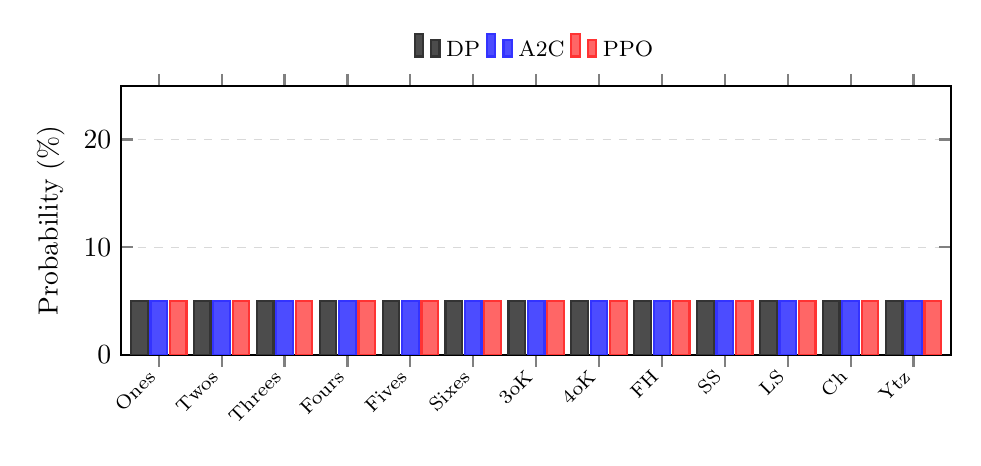
\begin{tikzpicture}
        \begin{axis}[
                ybar=1pt,
                width=\columnwidth,
                height=5cm,
                bar width=6pt,
                symbolic x coords={Ones,Twos,Threes,Fours,Fives,Sixes,3oK,4oK,FH,SS,LS,Ch,Ytz},
                xtick=data,
                xticklabel style={font=\scriptsize, rotate=45, anchor=east},
                ylabel={Probability (\%)},
                ymin=0,
                ymax=25,
                ymajorgrids=true,
                grid style={dashed,gray!30},
                legend style={
                        at={(0.5,1.05)},
                        anchor=south,
                        legend columns=3,
                        font=\footnotesize,
                        draw=none,
                        fill=none
                    },
                enlarge x limits=0.05,
                axis line style={thick},
                tick style={thick},
            ]

            % DP
            \addplot[fill=black!70, draw=black!80, thick] coordinates {
                    (Ones,5) (Twos,5) (Threes,5) (Fours,5) (Fives,5) (Sixes,5)
                    (3oK,5) (4oK,5) (FH,5) (SS,5) (LS,5) (Ch,5) (Ytz,5)
                };

            % A2C
            \addplot[fill=blue!70!white, draw=blue!80!white, thick] coordinates {
                    (Ones,5) (Twos,5) (Threes,5) (Fours,5) (Fives,5) (Sixes,5)
                    (3oK,5) (4oK,5) (FH,5) (SS,5) (LS,5) (Ch,5) (Ytz,5)
                };

            % PPO
            \addplot[fill=red!60!white, draw=red!80!white, thick] coordinates {
                    (Ones,5) (Twos,5) (Threes,5) (Fours,5) (Fives,5) (Sixes,5)
                    (3oK,5) (4oK,5) (FH,5) (SS,5) (LS,5) (Ch,5) (Ytz,5)
                };

            \legend{DP,A2C,PPO}

        \end{axis}
    \end{tikzpicture}
    \caption{First category chosen distribution (placeholder data)}
    \label{fig:strategy-first-category}
\end{figure}

\begin{figure}[H]
    \centering
    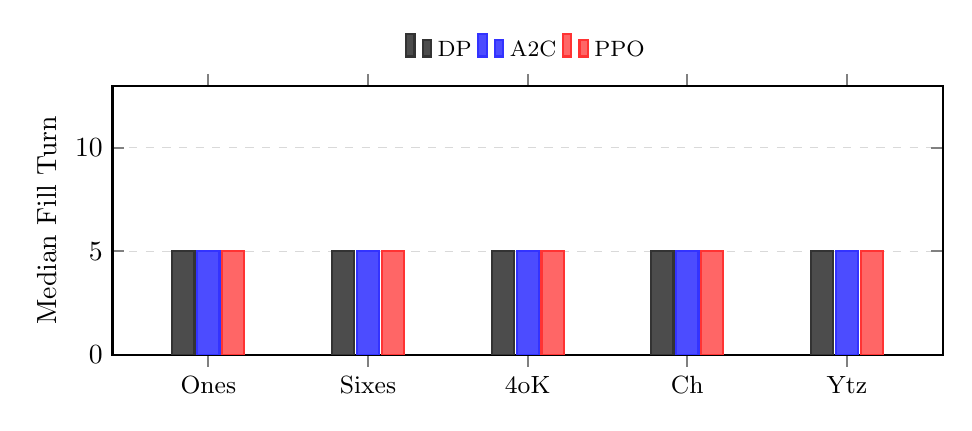
\begin{tikzpicture}
        \begin{axis}[
                ybar=1pt,
                width=\columnwidth,
                height=5cm,
                bar width=8pt,
                symbolic x coords={Ones,Sixes,4oK,Ch,Ytz},
                xtick=data,
                xticklabel style={font=\small},
                ylabel={Median Fill Turn},
                ymin=0,
                ymax=13,
                ymajorgrids=true,
                grid style={dashed,gray!30},
                legend style={
                        at={(0.5,1.05)},
                        anchor=south,
                        legend columns=3,
                        font=\footnotesize,
                        draw=none,
                        fill=none
                    },
                enlarge x limits=0.15,
                axis line style={thick},
                tick style={thick},
            ]

            % DP
            \addplot[fill=black!70, draw=black!80, thick] coordinates {
                    (Ones,5) (Sixes,5) (4oK,5) (Ch,5) (Ytz,5)
                };

            % A2C
            \addplot[fill=blue!70!white, draw=blue!80!white, thick] coordinates {
                    (Ones,5) (Sixes,5) (4oK,5) (Ch,5) (Ytz,5)
                };

            % PPO
            \addplot[fill=red!60!white, draw=red!80!white, thick] coordinates {
                    (Ones,5) (Sixes,5) (4oK,5) (Ch,5) (Ytz,5)
                };

            \legend{DP,A2C,PPO}

        \end{axis}
    \end{tikzpicture}
    \caption{Median fill turn for key categories (placeholder data)}
    \label{fig:strategy-fill-turn}
\end{figure}
